%Put this in order they appear in beamline?
\section{Beamline Components}

The Hall A Beamline has several measurement devices that allow the experimenter to fully understand the beam that is being delivered to the hall. For positioning, there are the Beam Position Monitors and the Harp. For beamspot sizing, there is the raster. For current and charge measurements, there are the Beam Current Monitors.

\subsection{Beam Position Monitors}

The Beam Position Monitors (BPMs) are a pair of measurement devices that consist of four sensing wires. By calibrating the signal received from each wire, the experimenter can reconstruct the position of the beam as it passed the BPM. Using both BPMs in conjunction allows the experimenter to determine the beam trajectory and where the electrons are incident on the target.

The BPMs are calibrated using a Harp fork. The Harp consists of three wires that are introduced sequentially into the path of the beam using a stepper motor. When the beam is incident on a wire, a charge is induced. By determining when each wire is struck by the beam, the experimenter can very accurately determine the position of the beam. This is an invasive measurement.

\subsection{Raster}
\begin{figure}
	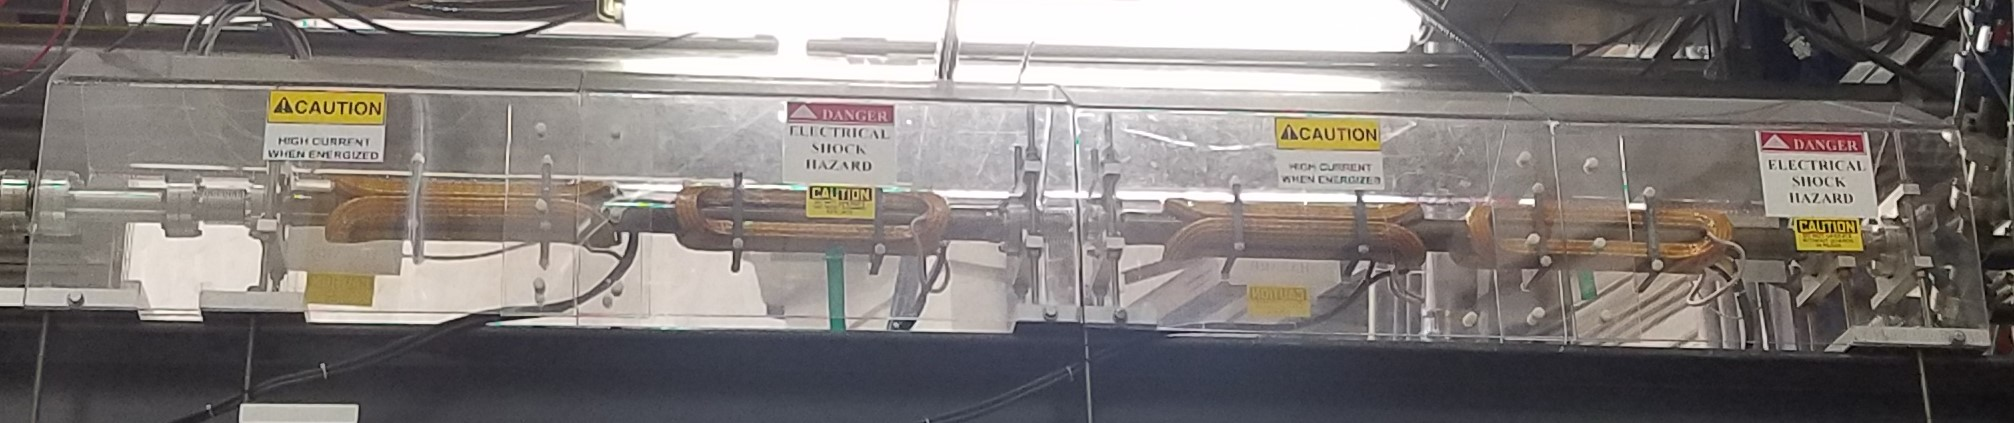
\includegraphics[width=\linewidth]{./chap2-exp/fig/raster_pic.jpg}
	\caption{The Hall A raster consists of four dipole magnets on the beamline}
	\label{fig:rasterpic}
\end{figure}

The raster is a beamline apparatus in Hall A for spreading the beam onto the target, rather than being at a single point. This is done to prevent localized heating of the target. The raster consists of four dipole magnets, two for steering in the x-direction and two for steering in the y-direction.

Each raster magnet is powered by a triangle wave of different frequencies to minimize harmonics. The horizontal rasters are set to 24.5 kHz and the vertical rasters are set to 25 kHz. When running properly, the x-direction magnets will be synced and the y-direction magnets will be synced. This syncing ensures that the magnets are always working together to create the desired beam spread.

\begin{figure}
	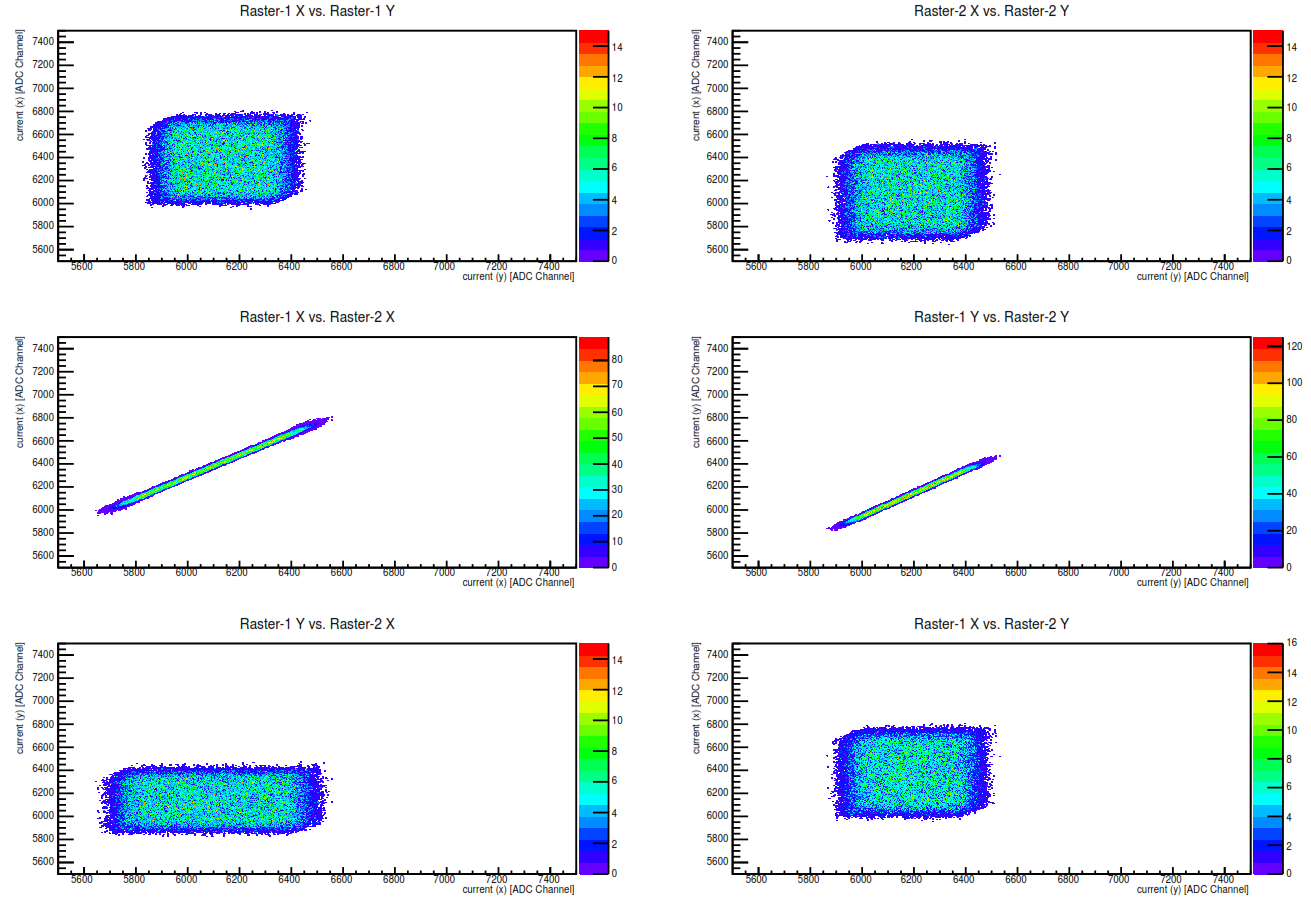
\includegraphics[width=\linewidth]{./chap2-exp/fig/raster_sync.png}
	\caption{The X and Y raster pairs are each synced to produce the maximum kick. The X and Y directions are uncorrelated so that the beam travels uniformly over the target.}
	\label{fig:raster}
\end{figure}

\subsection{Beam Current Monitors}